\ \ \ \ As we already construct the model and mathematical model that can calculate the chaos of the shop's layout, we are going to show that the created model is proper and can cause less damage to the products. 
\newline \par
Consider Figure 5.1 \& Figure 5.2
\begin{center}
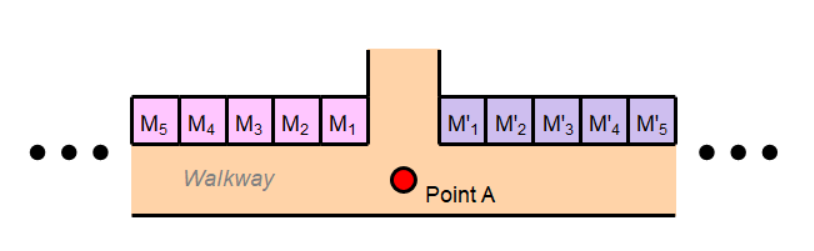
\includegraphics[width=\textwidth]{fig5.1.PNG}
Figure 8.1
\end{center}
\begin{center}
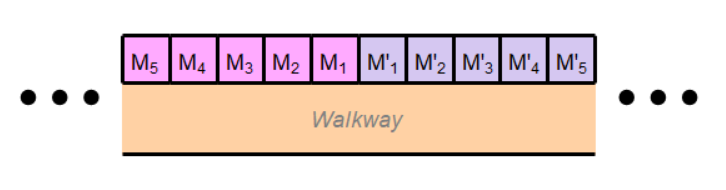
\includegraphics[width=\textwidth]{fig5.2.PNG}
Figure 8.2
\end{center}
\par
Now we are going to calculate the overall chaos value (that is related to store $M_1,M_2,\hdots,M_n$ and $M'_1,M'_2,\hdots,M'_n$) of the figure 8.1 and compare with figure 8.2.

The chaos of the figure 8.1 includes chaos of the walkway(caused by $M_1,M_2,\hdots,M_n$ and $M'_1,M'_2,\hdots,M'_n$) and the chaos of the intersection$_A$(caused by the row of store$_{M_1,M_2,\hdots,M_n}$ and row of store$_{M'_1,M'_2,\hdots,M'_n}$). The chaos of figure 8.2 contains only the chaos of walk way that is related to row of store$_{M_n,M_{n-1},M_{n-2},\hdots,M_2,M_1,M'_1,M'_2,\hdots,M'_n}$
Let the intersection$_A$ abbreviate as \emph{A}.
\newline
\newline
First, we calculate the chaos of the walkway.
\begin{enumerate}
    \item[] chaos of walkway$_{M_1,M_2,\hdots,M_n}=h_2$($M_1,M_n$)
    \item[] chaos of walkway$_{M'_1,M'_2,\hdots,M'_n}=h_2$($M'_1,M'_n$)
    \item[] chaos of walkway$_{M_n,M_{n-1},\hdots,M_2,M_1,M'_1,M'_2,\hdots,M'_n}$=$h_2$($M_n,M'_n$)
\end{enumerate}
\par
Then, we calculate the chaos of the intersection$_A$
\begin{enumerate}
    \item[] chaos of the intersection$_A=h_1$(row of store${_{M_n,M_{n-1},\hdots,M_1}}$,intersection$_A$) + $h_1$(row of store${_{M'_1,M'_2,\hdots,M'_n}}$,intersection$_A$)
\end{enumerate}
Let's define $H \equiv $ $h_1$(row of store$_{M_n,\hdots,M_1}$,\emph{A})
and 
$H' \equiv $ $h_1$(row of store$_{M'_n,\hdots,M'_1}$,\emph{A})

So it's enough to prove that 
\begin{center}
    $H$ + $H'$ + $h_2$($M_1,M_n$) + $h_2$($M'_1,M'_n$) $>$ $h_2$($M'_1,M'_n$)
\end{center}

\par
Let $\mathbb{M}$ be the set of all $M_{product}$
From $M_{product} \in (1,2)$, so for all $a,b,c \in \mathbb{M}$
We get that $a+b>1+1=2>c$.

Since $M_1,M_2,M'_1,M'_2\ \in \mathbb{M}$, then $M_1+M_2>M'_1$ and $M'_1+M'_2>M_1$
We get that
$M_1+\hdots+M_n\ >\ M_1+M_2\ >\ M'_1$ $\iff M_1M_2(M_1+\hdots+M_n)>M_1M_2M'_1$
\newline Therefore, we have
\begin{center}
    $M_1M_2(M_1+\hdots+M_n)>M_1M_2M'_1$ and $M'_1M'_2(M'_1+\hdots+M'_n)>M'_1M'_2M_1$
\end{center}

\begin{center}
$H$ + $H'$ $> M_1M_2M'_1+M'_1M'_2M_1$ 
\end{center}
\begin{center}
$\iff$
\end{center}
\begin{center}
$h_2$($M_1,M_n$) $ - M_1M_2+h_2$ ($M'_1,M'_n$) $ - M'_1M'_2+H$ + $H'$ $ > M_1M_2M'_1+M'_1M'_2M_1 + h_2$($M_1,M_n$)$ - M_1M_2+h_2$($M'_1,M'_n$)$ - M'_1M'_2$
\end{center}
\par
So $ h_2$($M_1,M_n$)$ + h_2$($M'_1,M'_n$)$ + H$ + $H'$ $ > h_2$($M'_1,M'_n$) as desired.
\par So we can conclude that if there exist two row of store connect to the same intersection, the chaos that related to all the store in these two row of store will be reduced when these two row of connect to each other. 
\par
In the similar way of proof, we can get that the chaos value related to store $M_1,M_2,\hdots M_n,M'_1,\hdots M'_n$ in figure 9.1 will be larger than in that the figure 9.2

\begin{center}
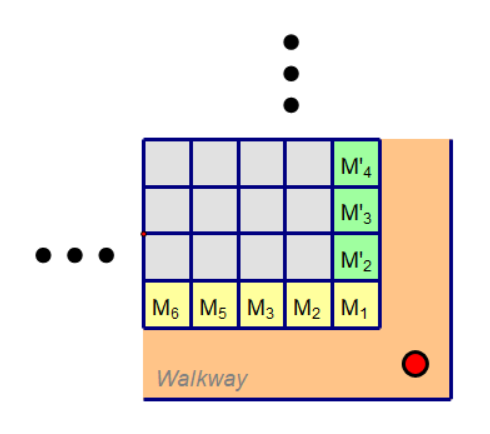
\includegraphics[width=0.7\textwidth]{fig6.1.PNG}
\end{center}
\begin{center}
Figure 9.1
\end{center}
\begin{center}
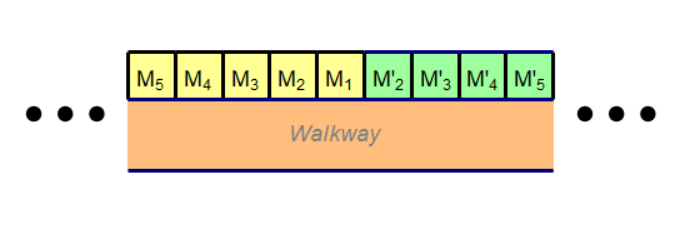
\includegraphics[width=\textwidth]{fig6.2.PNG}
\end{center}
\begin{center}
Figure 9.2
\end{center}

Therefore, if we connect two roles of store that either connect to the same intersection or perpendicular to each other(like figure 9.1) to be new long straight row of store, the new row of store will have lower chaos value.


When we consider the given layout, we can see many corners, which make the chaos of shop's layout to be high. We are going to show that it's able to find a chain from the layout such that this chain cover all the stores,in the condition that the same product type is adjacent, the same category is adjacent and the same department is adjacent. So if we use this new chain, called model \emph{L} to form a new layout of shop, like one long straight row of the store. [See figure 10 for an example of the chain], this long straight row(model \emph{L}) will has lower chaos value than the given layout as shown above.
\newline

Now we consider the model \emph{L}. As we have already mentioned(in solution and suggestion) that we use computer program to compile the permutation of the product in the linear layout, we get that the chaos value will be lower if there are more shopping lines of shelves.

Therefore, the given layout has higher chaos value than model \emph{L} and model \emph{L} has higher chaos than our proposed model, so the given layout also be more orderless and chaotic than our proposed model. Although we split the shopping mall into several shopping lines, we distribution all of the products to every shopping line equally to make sure that the spenders get the best shopping experience and choices to make, which will absolutely increase the spending probability and provide the host with more profits. Unfortunately, there exists a product which only is 5 item in quantity, so we can maximally split the shopping lanes into 5 lanes without losing economical advantages (in the amortized sense). From the computed data, we see that 5 lanes of shopping shelves provides good-enough result: doesn't significantly different to 6 or more lanes.

\begin{center}
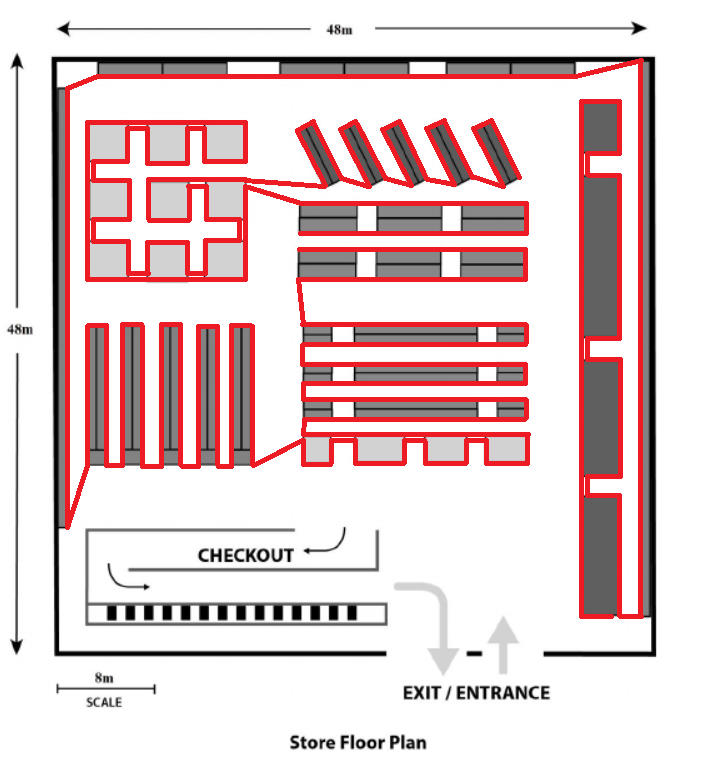
\includegraphics[width=\textwidth]{fig6.PNG}
Figure 10.
\end{center}